% !TEX root = ../thesis.tex
\section{Reflections \& Future Work}

\begin{figure}[b!]
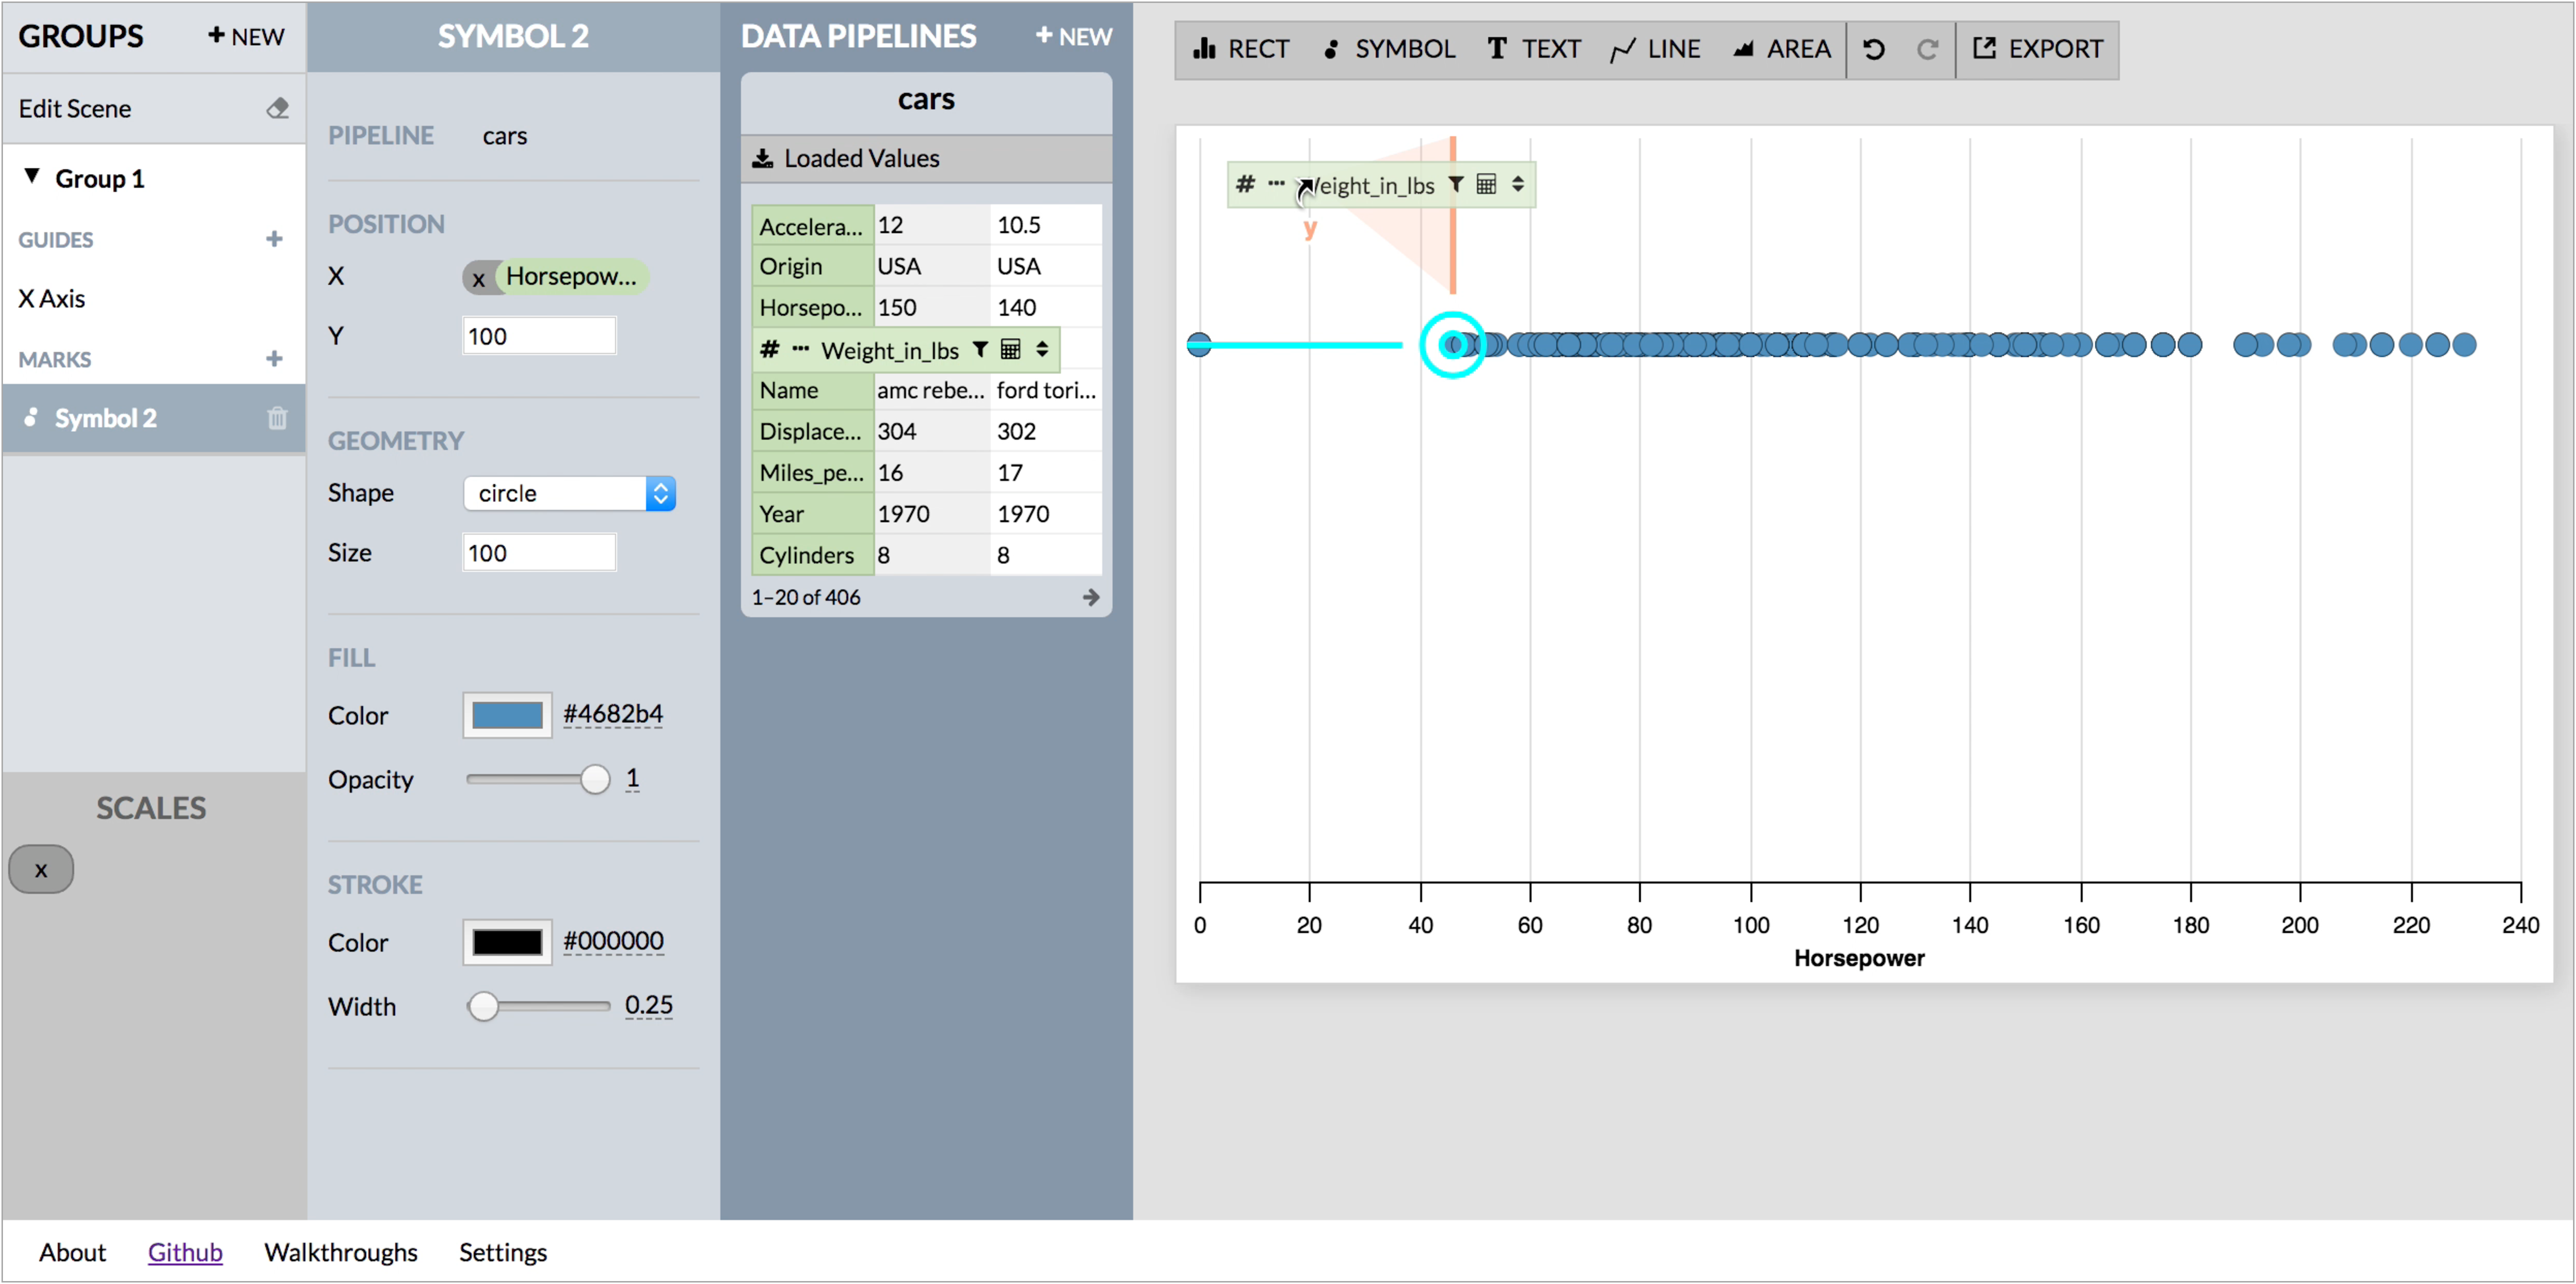
\includegraphics[width=\columnwidth]{lyra2}
\caption{The new Lyra interface. The side panels from \cref{fig:lyra:inspectors}
have been redesigned and consolidated to the left-hand side. As the user drags a
data field across the canvas, the nearest drop zone (highlighted in orange) is
automatically selected\,---\,a technique known as a bubble
cursor~\cite{grossman:bubble}.}
\label{fig:lyra2}
\end{figure}

Chronologically, Lyra was the first project to form part of this dissertation.
At the time of writing, a new version, that leverages Reactive Vega and
Vega-Lite, is under development. Thus, it is worth reflecting on how its role in
the ecosystem has evolved.

Much of Lyra's existing functionality can now be driven purely via a Reactive
Vega specification rather than through external callbacks. For instance, direct
manipulation operations on handles are now driven entirely via signals, rather
than event handling callbacks. Similarly, connectors make use of reactive
geometry directly. A bubble cursor~\cite{grossman:bubble} UDF (see
\cref{sec:udfs}) is registered to accelerate drop zone selection, as shown in
\cref{fig:lyra2}, addressing a major shortcoming users identified previously.

Moreover, Lyra's built-in production rule system has been subsumed by Vega-Lite.
Now, when users drag a data field onto a drop zone, a Vega-Lite unit
specification is compiled, the resultant Vega specification is statically
analyzed, and components selectively merged or updated in Lyra's backing Vega
specification.

With these changes, Lyra's place in the tool stack comes into sharper relief: it
\emph{bridges} two levels of abstraction within a single, cohesive environment.
Direct manipulation operations occur at the Vega-Lite level, and allow users to
rapidly generate recognizable visualizations. For more fine-grained
manipulation, or for custom design elements, users drop down to the Vega level
by interacting with the visual inspectors. A critical advantage of this approach
is that users can fluidly work with the level of abstraction best suited for the
task at hand. In fact, they may be altogether unaware of the separate roles
played by Vega and Vega-Lite under-the-hood!

Looking ahead, an exciting challenge is how Lyra might be extended to support
the design of \emph{interactive} visualizations. In-keeping with the above
approach, perhaps direct manipulation interactions (or demonstrations) should
generate Vega-Lite selections, which can be further modified with signal and
predicate inspectors.

Similarly, while Lyra's primary focus is currently on design tasks, data
visualization inevitably requires data cleaning and transformation. Lyra's data
pipelines offer sufficient flexibility to support analytic tasks, but require
familiarity with transformation operators. Can direct manipulation methods, akin
to those in Data Wrangler~\cite{kandel:wrangler}, be further incorporated to
specify more complex data transformations?